\documentclass[french,11pt,a4paper,twoside,openright]{report}
% openright chap sur page de droite
\usepackage[left=2cm,right=2cm,top=2cm,bottom=2cm]{geometry}
\usepackage[utf8x]{inputenc}
\usepackage[T1]{fontenc}
\usepackage{xcolor}
\usepackage[english,frenchb]{babel}
\usepackage{amsmath}
\usepackage{amsfonts}
\usepackage{amssymb}
\usepackage{bbm}
\usepackage{graphicx}
\usepackage[font={normalsize},labelfont={normalsize},figurename=Figure,tablename=Tableau,center]{caption}
\usepackage[lofdepth,lotdepth]{subfig}
\usepackage{booktabs}
\usepackage{fancyhdr}
\setlength\heavyrulewidth{1.0pt}
\usepackage{epigraph}
\usepackage{placeins}
\usepackage{floatrow}
\floatsetup[table]{capposition=top}
\usepackage[linkcolor=blue]{hyperref} 
\hypersetup{                    % parametrage des hyperliens
    colorlinks=true,                % colorise les liens
    breaklinks=true,                % permet les retours à la ligne pour les liens trop longs
    urlcolor= blue,                 % couleur des hyperliens
    linkcolor= black,                % couleur des liens internes aux documents (index, figures, tableaux, equations,...)
    citecolor= red                % couleur des liens vers les references bibliographiques
    }
\usepackage[frenchb]{minitoc}		% Mini table des matières, en français
\setcounter{minitocdepth}{2}	% Mini-toc détaillées (sections/sous-sections)
\setcounter{tocdepth}{3}
\setcounter{secnumdepth}{3}
%\usepackage[pdftex]{graphicx}

% police demandee par le CEA, a decommenter pour utiliser

%\usepackage{helvet}
%\renewcommand{\familydefault}{\sfdefault}

% Tracé de figures vectorielles
\usepackage{tikz}
\usepackage{pgfkeys}
\usepackage{pgfplots}
% Formules chimiques
\usepackage{chemfig}
\usepackage{mhchem}
% Gestion des unites
\usepackage{eurosym}
\usepackage{siunitx} % écriture des unités
\sisetup{detect-all} % permet de mettre en gras les unités avec txbf
\sisetup{locale=FR} % permet de reconnaître les règles syntaxiques françaises
\sisetup{inter-unit-product=\ensuremath{\cdot}} % permet de changer le formalisme du multiplier

\usepackage{import}

\newcommand{\citationChap}[2]{                    % commande pour les citations
	\epigraph{\og \textit{#1} \fg{}}{#2}
}

% Definition de la couleur verte pour la première page
\usepackage{colortbl}
\definecolor{darkgreen}{cmyk}{0.7,0,0.7,0.5}
\definecolor{darkred}{rgb}{0.8,0,0}
\newcommand{\HRule}{\rule{\linewidth}{0.5mm}}

\newcommand\ytl[3]{
\parbox[b]{8em}{\hfill{\color{#3}\bfseries\sffamily #1}~$\cdots\cdots$~}\makebox[0pt][c]{$\bullet$}\vrule\quad \parbox[c]{4.5cm}{\vspace{7pt}\color{red!40!black!80}\raggedright\sffamily #2.\\[7pt]}\\[-3pt]
}




% Macros utiles dans ce document

%
% Abreviations utilisees dans le texte
%

\def\cel{cellulose}

%
% Abreviation de mots accentues courants
%

\def\a{\`a}
\def\abinitio{{\it ab initio\/}}
\def\aposteriori{{\it a posteriori\/}}
\def\apriori{{\it a priori\/}}
\def\ca{\c ca}
\def\cote{c\^ot\'e}
\def\chaine{cha\^ine}
\def\deja{d\'ej\`a}
\def\dela{del\`a}
\def\du{d\^u}
\def\etc{{\it etc\/}}
\def\ete{\'et\'e}
\def\etre{\^etre}
\def\grace{gr\^ace}
\def\la{l\`a}
\def\laou{l\`a o\`u}
\def\lache{l\^ache}
\def\meme{m\^eme}
\def\Meme{M\^eme}
\def\noeud{n\oe ud}
\def\ou{o\`u}
\def\quasi{{\it quasi\/}}
\def\role{r\^ole}

%
% Abreviation de caracteres usuels
%

% degre
\def\dg{$^\circ$}
\def\scdg{$\scrp^\circ$}
\def\dgm{^\circ}
\def\dgc{\dg C}

% paragraphe
\def\Sb#1{\S\kern .15em #1}


			% macros specifiques a ce document
% Alphabet grec : raccourcis
%
% Il reste a coder le KHI en remontant le minuscule. \up ne marche pas car il remonte toute la ligne apres.
% pour le moment, c'est code par un X
%
\def\alp{\alpha}
\def\bet{\beta}
\def\gam{\gamma} 
\def\del{\delta} 
\def\eps{\epsilon}
\def\veps{\varepsilon}
\def\dze{\zeta}
\def\tet{\theta}
\def\vtet{\vartheta}
\def\iot{\iota}
\def\kap{\kappa}
\def\lam{\lambda}
\def\ksi{\xi}
\def\omi{o}
\def\vpi{\varpi}
\def\vrho{\varrho}
\def\sig{{\sigma}}
\def\vsig{\varsigma}
\def\ups{\upsilon}
\def\vphi{\varphi}
\def\khi{\chi}
\def\ome{\omega}
\def\Alp{{\rm A}}
\def\Bet{{\rm B}}
\def\Gam{\Gamma} 
\def\Del{\Delta} 
\def\Eps{{\rm E}}
\def\Dze{{\rm Z}}
\def\Eta{{\rm H}}
\def\Tet{\Theta}
\def\Iot{{\rm I}}
\def\Kap{{\rm K}}
\def\Lam{\Lambda}
\def\Mu{{\rm M}}
\def\Nu{{\rm N}}
\def\Ksi{\Xi}
\def\Omi{{\rm O}}
\def\Rho{{\rm P}}
\def\Sig{{\Sigma}}
\def\Tau{{\rm T}}
\def\Ups{\Upsilon}
\def\Khi{\rm X}
\def\Ome{\Omega}
		% macros specifiques a ce document
%
% macros d'insertions de figures
%

%
% macro de numerotation	des figures
%

%% definition du compteur de figures			
%\newcount\numfig \numfig=0								% avec_numerotation
%\def\fig{\global\advance\numfig by 1{\bfuit figure~\the\numfig :} \rmuit}		% avec_numerotation
%%\def\fig{fig }										% sans_numerotation
% 
%% macros de referencage des figures			
%
%% referencage manuel					
%%\def\fignum#1{(fig~#1)}								% sans_numerotation
%
%% referencage automatique								% avec_numerotation
%% (attention a ne pas introduire de blancs parasites)					% avec_numerotation
%% Une figure en haut/en bas								% avec_numerotation
%\def\figh{                     (fig \the\numfig)}				% avec_numerotation
%\def\figb{\advance\numfig by 1	(fig~\the\numfig)\advance\numfig by -1}	% avec_numerotation
%% Deux fig en haut/bas et on veut celle de gauche/droite				% avec_numerotation
%\def\dfighg{\advance\numfig by -1(fig~\the\numfig)\advance\numfig by 1}	% avec_numerotation
%\def\dfighd{                     (fig~\the\numfig)}			% avec_numerotation
%\def\dfigbg{\advance\numfig by 1 (fig~\the\numfig)\advance\numfig by -1}	% avec_numerotation
%\def\dfigbd{\advance\numfig by 2 (fig~\the\numfig)\advance\numfig by -2}	% avec_numerotation
%% Deux fig en haut/bas et on veut les deux						% avec_numerotation
%\def\dfigb{\advance\numfig by 1(fig~\the\numfig%				% avec_numerotation
%  \advance\numfig by 1\&~\the\numfig)\advance\numfig by -2}		% avec_numerotation
%\def\dfigh{\advance\numfig by -1(fig~\the\numfig%				% avec_numerotation
%  \advance\numfig by 1\&~\the\numfig)}					% avec_numerotation
%% Trois fig en haut/bas  et on veut celle de gauche/milieu/droite			% avec_numerotation
%\def\tfighg{\advance\numfig by -2(fig~\the\numfig)\advance\numfig by 2}	% avec_numerotation
%\def\tfighm{\advance\numfig by -1(fig~\the\numfig)\advance\numfig by 1}	% avec_numerotation
%\def\tfighd{                     (fig~\the\numfig)}			% avec_numerotation
%\def\tfigbg{\advance\numfig by 1 (fig~\the\numfig)\advance\numfig by -1}	% avec_numerotation
%\def\tfigbm{\advance\numfig by 2 (fig~\the\numfig)\advance\numfig by -2}	% avec_numerotation
%\def\tfigbd{\advance\numfig by 3 (fig~\the\numfig)\advance\numfig by -3}	% avec_numerotation
%% Trois fig en haut/bas  et on veut les trois						% avec_numerotation
%\def\tfigb{\advance\numfig by 1(fig~\the\numfig,%				% avec_numerotation
%  \advance\numfig by 1~\the\numfig~\&% 					% avec_numerotation
%  \advance\numfig by 1~\the\numfig)\advance\numfig by -3}			% avec_numerotation
%\def\tfigh{\advance\numfig by -2(fig~\the\numfig,%			% avec_numerotation
%  \advance\numfig by 1~\the\numfig~\&%					% avec_numerotation
%  \advance\numfig by 1~\the\numfig)}					% avec_numerotation

\def\figp#1{(figure~\ref{#1})}
\def\fig#1{figure~\ref{#1}}

%-----------------------------------------------------------
%-----------------------------------------------------------
%-----------------------------------------------------------

%
% procedures pour inclure des fichiers postscript encapsules 
%     (les unites sont a preciser avec les dimensions)
%

\def\sfigx#1#2{\hbox{\epsfxsize=#1\epsffile{#2.eps}}}
\def\sfigy#1#2{\hbox{\epsfysize=#1\epsffile{#2.eps}}}
\def\sfigxy#1#2#3{\hbox{\epsfxsize=#1\epsfysize=#2\epsffile{#3.eps}}}



%-----------------------------------------------------------
%
% figx : insertion d'un fichier redimensionne en x
%
% #1 = dimension suivant x du dessin
% #2 = nom du fichier a inserer sans l'extension ".eps"
% #3 = legende
% #4 = position de la legende
% #5 = decalage vertical avant
% #6 = decalage vertical apres
%

\def\figx#1#2#3#4#5#6#7{
%  \vskip#4  	 			% decalage
%  \vbox{                             	% ouverture d'une boite V
%    {\ \hfill\sfigx{#1}{#2}\hfill}	% centrage de la figure
%    \vskip#5   	 			% decalage
%    \centerline{\fig #3}             	% centrage d'une legende	
%  }                             	% fermeture d'une boite V
%  \vskip#6				% decalage
 \begin{figure}
  \begin{center}
   \includegraphics[width=#1]{#2.eps}
  \end{center}
  \caption{#3}
  \label{#7}
 \end{figure}
}        		                         

%-----------------------------------------------------------
%
% figxy : insertion d'un fichier redimensionne en x et y
%
% #1 = dimension suivant x du dessin
% #2 = dimension suivant y du dessin
% #3 = nom du fichier a inserer sans l'extension ".eps"
% #4 = legende
% #5 = position de la legende
% #6 = decalage vertical avant
% #7 = decalage vertical apres
%

\def\figxy#1#2#3#4#5#6#7{
  \vskip#5  	 			% decalage
  \vbox{                             	% ouverture d'une boite V
    {\ \hfill\sfigxy{#1}{#2}{#3}\hfill}       % centrage de la figure
    \vskip#6   	 			% decalage
%    \centerline{\fig #4}             	% centrage d'une legende	
  }                             	% fermeture d'une boite V
  \vskip#7				% decalage
}        		                        

%-----------------------------------------------------------
%
% dfigx : insertion de deux figures de meme taille en x 
%         (les unites sont a preciser aves les dimensions)
%
% #1 = dimension suivant x des deux figures      
% #2 = nom du fichier de gauche sans l'extension ".eps"
% #3 = nom du fichier de droite sans l'extension ".eps"
% #4 = legende de gauche 
% #5 = legende de droite 
% #6 = position verticale des legendes
% #7 = decalage vertical avant
% #8 = decalage vertical apres
%

\newdimen\largeur 							

\def\dfigx#1#2#3#4#5#6#7#8{
  \largeur=\textwidth \divide\largeur by2 \advance\largeur by-1truept 	
  \setbox101=\sfigx{#1}{#2}
  \setbox102=\sfigx{#1}{#3}
%  \setbox104=\hbox to \largeur{\hfill\hbox{\fig #4}\hfill}	
%  \setbox105=\hbox to \largeur{\hfill\hbox{\fig #5}\hfill}	
  \vbox{
    \vskip #7
    \hbox to \textwidth{\hfill\box101\hfill\box102\hfill}
    \vskip #6
%    \hbox to \textwidth{\hfill\box104\hfill\box105\hfill}
    \vskip #8
    }
}

%-----------------------------------------------------------
%
% dfigxiso : insertion de deux figures en ligne de dimensions differentes
%            chacune centree dans sa moitie de la page
%         (les unites sont a preciser aves les dimensions)
%
% #1 = dimension suivant x de la figure de gauche
% #2 = dimension suivant x de la figure de droite   
% #3 = nom du fichier de gauche sans l'extension ".eps"
% #4 = nom du fichier de droite sans l'extension ".eps"
% #5 = legende de gauche 
% #6 = legende de droite 
% #7 = position verticale des legendes
% #8 = decalage vertical avant
% #9 = decalage vertical apres
%
\def\dfigxiso#1#2#3#4#5#6#7#8#9{
  \largeur=\textwidth \divide\largeur by2 \advance\largeur by-1truept 	
  \setbox101=\sfigx{#1}{#3}
  \setbox102=\sfigx{#2}{#4}
  \setbox101=\hbox to \largeur{\hfill\box101\hfill}
  \setbox102=\hbox to \largeur{\hfill\box102\hfill}
%  \setbox104=\hbox to \largeur{\hfill\hbox{\fig #5}\hfill}	
%  \setbox105=\hbox to \largeur{\hfill\hbox{\fig #6}\hfill}	
  \vbox{
    \vskip #8
    \hbox to \textwidth{\hfill\box101\hfill\box102\hfill}
    \vskip #7
    \hbox to \textwidth{\hfill\box104\hfill\box105\hfill}
    \vskip #9
    }
}

%-----------------------------------------------------------
%
% dfigxdif : insertion de deux figures en ligne de dimensions differentes
%            avec les blancs repartis egalement entre les figures
%         (les unites sont a preciser aves les dimensions)
%
% #1 = dimension suivant x de la figure de gauche
% #2 = dimension suivant x de la figure de droite   
% #3 = nom du fichier de gauche sans l'extension ".eps"
% #4 = nom du fichier de droite sans l'extension ".eps"
% #5 = legende de gauche 
% #6 = legende de droite 
% #7 = position verticale des legendes
% #8 = decalage vertical avant
% #9 = decalage vertical apres
%

\def\dfigxdif#1#2#3#4#5#6#7#8#9{
  \setbox101=\sfigx{#1}{#3}
  \setbox102=\sfigx{#2}{#4}
%  \setbox104=\hbox to #1{\hfill\hbox{\fig #5}\hfill}	
%  \setbox105=\hbox to #2{\hfill\hbox{\fig #6}\hfill}	
  \vbox{
    \vskip #8
    \hbox to \textwidth{\hfill\box101\hfill\box102\hfill}
    \vskip #7
%    \hbox to \textwidth{\hfill\box104\hfill\box105\hfill}
    \vskip #9
    }
}

%-----------------------------------------------------------
%
% tfigx : insertion de trois figures de meme dimension 
%         (les unites sont a preciser aves les dimensions)
%
% #1 = dimension suivant x de la figure de gauche
% #2 = nom du fichier de gauche sans l'extension ".eps"
% #3 = nom du fichier du centre sans l'extension ".eps"
% #4 = nom du fichier de droite sans l'extension ".eps"
% #5 = legendes de l'image de gauche
% #6 = legendes de l'image du milieu
% #7 = legendes de l'image de droite
% #8 = decalage vertical avant
% #9 = decalage vertical apres
%

\def\tfigx#1#2#3#4#5#6#7#8#9{
  \largeur=\textwidth \divide\largeur by3 \advance\largeur by-1truept 	
  \setbox101=\sfigx{#1}{#2}
  \setbox102=\sfigx{#1}{#3}
  \setbox103=\sfigx{#1}{#4}
  \setbox101=\hbox to \largeur{\hfill\box101\hfill}
  \setbox102=\hbox to \largeur{\hfill\box102\hfill}
  \setbox103=\hbox to \largeur{\hfill\box103\hfill}
%  \setbox104=\hbox to \largeur{\hfill\hbox{\fig #5}\hfill}	
%  \setbox105=\hbox to \largeur{\hfill\hbox{\fig #6}\hfill}	
%  \setbox106=\hbox to \largeur{\hfill\hbox{\fig #7}\hfill}	
  \vbox{
    \vskip #8
     \hbox to \textwidth{\hfill\box101\hfill\box102\hfill\box103\hfill}
     \vskip 2mm
%     \hbox to \textwidth{\hfill\box104\hfill\box105\hfill\box106\hfill}
     \vskip #9
    }
}

%-----------------------------------------------------------
%
% tfigxiso : insertion de trois figures en ligne de dimension et de legendes differentes 
%            chacune centree dans sa moitie de la page
%         (les unites sont a preciser aves les dimensions)
%
% #1 = dimension suivant x de la figure de gauche
% #2 = dimension suivant x de la figure du milieu
% #3 = dimension suivant x de la figure de droite
% #4 = nom du fichier de gauche sans l'extension ".eps"
% #5 = nom du fichier du centre sans l'extension ".eps"
% #6 = nom du fichier de droite sans l'extension ".eps"
% #7 = legendes de l'image de gauche 
% #8 = legendes de l'image du milieu
% #9 = legendes de l'image de droite
%

\def\tfigxiso#1#2#3#4#5#6#7#8#9{
  \largeur=\textwidth \divide\largeur by3 \advance\largeur by-1truept 	
  \setbox101=\sfigx{#1}{#4}
  \setbox102=\sfigx{#2}{#5}
  \setbox103=\sfigx{#3}{#6}
  \setbox101=\hbox to \largeur{\hfill\box101\hfill}
  \setbox102=\hbox to \largeur{\hfill\box102\hfill}
  \setbox103=\hbox to \largeur{\hfill\box103\hfill}
%  \setbox104=\hbox to \largeur{\hfill\hbox{\fig #7}\hfill}	
%  \setbox105=\hbox to \largeur{\hfill\hbox{\fig #8}\hfill}	
%  \setbox106=\hbox to \largeur{\hfill\hbox{\fig #9}\hfill}	
  \vbox{
    \vskip 2mm
     \hbox to \textwidth{\hfill\box101\hfill\box102\hfill\box103\hfill}
     \vskip 2mm
%     \hbox to \textwidth{\hfill\box104\hfill\box105\hfill\box106\hfill}
     \vskip 0mm
    }
}

%-----------------------------------------------------------
%
% tfigxiso : insertion de trois figures en ligne de dimension et de legendes differentes 
%            avec les blancs repartis egalement entre les figures
%         (les unites sont a preciser aves les dimensions)
%
% #1 = dimension suivant x de la figure de gauche
% #2 = dimension suivant x de la figure du milieu
% #3 = dimension suivant x de la figure de droite
% #4 = nom du fichier de gauche sans l'extension ".eps"
% #5 = nom du fichier du centre sans l'extension ".eps"
% #6 = nom du fichier de droite sans l'extension ".eps"
% #7 = legendes de l'image de gauche 
% #8 = legendes de l'image du milieu
% #9 = legendes de l'image de droite
%

\def\tfigxdif#1#2#3#4#5#6#7#8#9{
  \setbox101=\sfigx{#1}{#4}
  \setbox102=\sfigx{#2}{#5}
  \setbox103=\sfigx{#3}{#6}
  \setbox104=\hbox to #1{\hfill\hbox{\fig #7}\hfill}	
  \setbox105=\hbox to #2{\hfill\hbox{\fig #8}\hfill}	
  \setbox106=\hbox to #3{\hfill\hbox{\fig #9}\hfill}	
  \vbox{
    \vskip 2mm
     \hbox to \textwidth{\hfill\box101\hfill\box102\hfill\box103\hfill}
     \vskip 2mm
     \hbox to \textwidth{\hfill\box104\hfill\box105\hfill\box106\hfill}
     \vskip 2mm
    }
}


%-----------------------------------------------------------
%-----------------------------------------------------------
%-----------------------------------------------------------

%
% macros d'insertion de tableaux
%


 % definition du compteur de tableaux			% avec_numerotation
%\newcount\numtab \numtab=0				% avec_numerotation
%
%% % macro de numerotation					% numerotation
%%\def\tabn#1{tab~#1 :}						% sans_numerotation
%\def\tabn{\global\advance\numtab by 1 				% avec_numerotation
%%	\rmuit							% avec_numerotation
%	TABLEAU~\the\numtab : }			% avec_numerotation
% 
%% % macros de referencage des tableaux				% numerotation
%
%% % referencage manuel						% sans_numerotation
%%\def\tac#1{(tac~#1)}						% sans_numerotation
%
% % referencage automatique					% avec_numerotation
% % le tableau est en haut					% avec_numerotation
%\def\tabh{tableau~\the\numtab}			% avec_numerotation
% % le tableau est deux tableaux avant				% avec_numerotation
%\def\tabhh{{\advance\numtab by -1%				% avec_numerotation
%tableau~\the\numtab}}		% avec_numerotation
% % le tableau est en bas					% avec_numerotation
%\def\tabb{{\advance\numtab by 1%				% avec_numerotation
%tableau~\the\numtab}}		% avec_numerotation
% % le tableau est deux tableaux en bas				% avec_numerotation
%\def\tabbb{{\advance\numtab by 2%				% avec_numerotation
%tableau~\the\numtab}}		% avec_numerotation

\def\tabp#1{(tableau~\ref{#1})}
\def\tab#1{tableau~\ref{#1}}

%-----------------------------------------------------------

%
% insertion de tableau
% les unites sont a preciser avec les dimensions
% 
% #1 le titre
% #2 le tableau
% #3 commentaire eventuel
% #4 ecart entre le titre et le tableau
% #5 ecart entre le tableau et le commentaire
% #6 ecart avant le tableau 
% #7 ecart apres le tableau
%

\def\tableau#1#2#3#4#5#6#7#8{
   \begin{table}
 	\vbox{
%		\setbox100=\ctitre{#1}		% sans_numerotation
%		\setbox100=\ctitre{\caption{#1}\label{#8}}	% avec_numerotation
		\setbox101=\vbox{#2}
		\setbox102=\ctitre{#3}

		\vskip #6 
%		\centerline{\box100}
                \caption{#1}\label{#8}
		\vglue #4 plus 2pt minus 2pt 
		\centerline{\box101}
		\vglue #5 plus 2pt minus 2pt 
		\centerline{\box102}
		\vskip #7
	}
   \end{table}
}




  		% macros specifiques a ce document
%
% macros definies dans "Le Petit Livre De TeX de Raymond Seroul"
%

\catcode`\@=11 	% le temps de tout definir, c'est un caractere.

%
% note de bas de page (Ch. 6 : page 85)
% \note{texte}

\newcount\notenumber \notenumber=1
\def\note#1{\footnote{$^{\the\notenumber}$}{#1}%
\global\advance\notenumber by 1}

% 
% centrer un titre (Index : page 238)
% 

\long\def\ctitre#1{\vbox{\leftskip=0pt plus 1fil \rightskip=0pt plus 1fil \parfillskip=0pt #1}}

%
% pour faire un sommaire
%

\def\page#1{\leaders\hbox to 5mm{\hfil.\hfil}\hfill\rlap{\hbox to 10mm{\hfill#1}}\par}

% 
% pour les tableaux (Ch. 9 : Les tableaux)
% 

% traits verticaux invisibles et visibles
\def\tvi{\vrule height 12pt depth 5pt width 0pt}
\def\Tvi#1{ 	\ifnum #1=0	\vrule height  4pt depth 1pt width 0pt  \fi
	 	\ifnum #1=1	\vrule height 10pt depth 3pt width 0pt  \fi
	   	\ifnum #1=2	\vrule height 11pt depth 4pt width 0pt  \fi
	   	\ifnum #1=3	\vrule height 12pt depth 5pt width 0pt  \fi
	   	\ifnum #1=4	\vrule height 13pt depth 5pt width 0pt  \fi
	   	\ifnum #1=5	\vrule height 14pt depth 6pt width 0pt  \fi
	   	\ifnum #1=6	\vrule height 48pt depth 20pt width 0pt  \fi
	   }	
\def\tv{\tvi\vrule}
\def\Tv#1{\Tvi#1\vrule}

\def\hfq{\hfill\quad}  
\def\qhf{\quad\hfill}  
%pour centrer avec un quadratin a dte et a gche
\def\cc#1{\hfill\quad#1\quad\hfill}  
%pour centrer avec un demi quadratin a dte et a gche
\def\dd#1{\hfill\enspace#1\enspace\hfill}
%pour centrer avec un espace a dte et a gche
\def\ee#1{\hfill\ #1\ \hfill} 
%pour centrer sans rien  a dte ni a gche
\def\ff#1{\hfill #1\hfill} 

%%
%% guillemets francais
%%
%\def\og{\leavevmode\raise.3ex\hbox{$\scriptscriptstyle\langle\!\langle\,$}}
%\def\osg{\leavevmode\raise.3ex\hbox{$\scriptscriptstyle\langle\,$}}
%\def\fg{\leavevmode\raise.3ex\hbox{$\scriptscriptstyle\,\rangle\!\rangle$}}
%\def\fsg{\leavevmode\raise.3ex\hbox{$\scriptscriptstyle\,\rangle$}}
\def\ogui{\leavevmode\raise.3ex\hbox{$\scriptscriptstyle\langle\!\langle\,$}}
\def\fgui{\leavevmode\raise.3ex\hbox{$\scriptscriptstyle\,\rangle\!\rangle$}}

% numerotation romaine
\def\numrom#1{\uppercase\expandafter{\romannumeral #1 }}

% numerotation ancien style (utilise pour les annees, par exemple)
\let\an=\oldstylenums

% etoile en mode non mathematique
\def\stern{$\star$}

% pour les exposants et indices en mode non mathematique (chap 12 p217)

\def\up#1{\raise 1ex\hbox{\rmneu #1}}
\def\dw#1{\raise -0.5ex\hbox{\rmneu #1}}
\def\ind#1{\dw{\rmset #1}}

%
% lettrine
% #1 largeur indentee
% #2 nb de lignes a indenter
% #3 lettres a inserer
% \lettrine{30mm}{4}{L}'homme etc

\def\lettrine#1#2#3{\noindent\hangindent#1\hangafter-#2
		    \hskip-#1\smash{\hbox to#1{#3\hfill}}\ignorespaces}


%
% entourer une boite #2 d'un liseret d'epaisseur #1 (qq pt) page 123
% \boxit{qq pt}{la boite contenant le texte}
% \boxitxy permet de specifier un ecart different en x et en y
% \trait trace juste un trait a gauche de la boite 

\def\boxit#1#2{\setbox1=\hbox{\kern#1{#2}\kern#1}%
\dimen1=\ht1 \advance\dimen1 by #1 \dimen2=\dp1 \advance\dimen2 by #1
\setbox1=\hbox{\vrule height\dimen1 depth\dimen2\box1\vrule}%
\setbox1=\vbox{\hrule\box1\hrule}%
\advance\dimen1 by .4pt \ht1=\dimen1
\advance\dimen2 by .4pt \dp1=\dimen2 \box1\relax}

\def\boxitxy#1#2#3{\setbox1=\hbox{\kern#1{#3}\kern#1}%
\dimen1=\ht1 \advance\dimen1 by #2 \dimen2=\dp1 \advance\dimen2 by #2
\setbox1=\hbox{\vrule height\dimen1 depth\dimen2\box1\vrule}%
\setbox1=\vbox{\hrule\box1\hrule}%
\advance\dimen1 by .4pt \ht1=\dimen1
\advance\dimen2 by .4pt \dp1=\dimen2 \box1\relax}

\def\trait#1#2{\setbox1=\vbox{\kern#1{#2}\kern#1}%
\dimen1=\ht1 \advance\dimen1 by #1 \dimen2=\dp1 \advance\dimen2 by #1
\setbox1=\hbox{\vrule height\dimen1 depth\dimen2\box1}%
\box1\relax}

%
% pour ajouter des choses au dessus ou en dessous d'un symbole mathematique
%

\def\build#1#2^#3{\mathrel{\mathop{\kern 0pt#1}\limits_{#2}^{#3}}}

%
% systeme d'equations : page 192
%

\def\system#1{\left\{\null\,\vcenter{\openup1\jot\m@th
\ialign{\strut\hfil$##$&$##$\hfil&&\enspace$##$\enspace&
\hfil$##$&$##$\hfil\crcr#1\crcr}}\right.}

%
% diagram page 190 (autre version dans le ed2 p 160.)
%
\def\hfl#1#2{\smash{\mathop{\hbox to 12mm{\rightarrowfill}}\limits^{\scriptstyle #1}_{\scriptstyle #2}}}
\def\hlf#1#2{\smash{\mathop{\hbox to 12mm{\leftarrowfill}}\limits^{\scriptstyle #1}_{\scriptstyle #2}}}
\def\vfl#1#2{\llap{$\scriptstyle #1$}\left\downarrow\vbox to 6mm{}\right.\rlap{$\scriptstyle #2$}}
\def\vlf#1#2{\llap{$\scriptstyle #1$}\left\uparrow\vbox to 6mm{}\right.\rlap{$\scriptstyle #2$}}
\def\diagram#1{\def\normalbaselines{\baselineskip=0pt\lineskip=10pt\lineskiplimit=1pt} \matrix{#1}}

%
% Eqalign, version modifi\'ee de equalign
%
\def\Eqalign#1{\null\,\vcenter{\openup\jot\m@th\ialign{
\strut\hfil$\displaystyle{##}$&$\displaystyle{{}##}$\hfil&&\quad
\strut\hfil$\displaystyle{##}$&$\displaystyle{{}##}$\hfil\crcr#1\crcr}}\,}

%
% EEqalign. comme system, mais sans l'accolade.
%
\def\EEqalign#1{\left.\null\,\vcenter{\openup1\jot\m@th
\ialign{\strut\hfil$##$&$##$\hfil&&\enspace$##$\enspace&
\hfil$##$&$##$\hfil\crcr#1\crcr}}\right.}

%
% ecriture sur deux colonnes (TeXbook p417) 10 9bre 2
%
%  emploi :
%  \begindoublecolumns
%   texte
%  \enddoublecolumns
%
% Si on veut preciser soit meme la largeur des colonnes, il faut ecrire
% \begindoublecolumnsdim{N}, ou N est la largeur en mm que l'on desire donner a la colonne.
%
% Remarque : 
%  1) il y une autre solution pour ecrire avec deux colonnes : voir le
% TeXbook p257. cette solution permet aussi d'ecrire sur 3 colonnes
%  2) cette macro gere les notes de bas de page, mais les met en bas en colonne unique.
%     D. Knuth propose de faire � titre d'exercice la modification pour associer
%     a chaque colonne ses notes de bas de page

\newdimen\pagewidth \pagewidth=\hsize
\newbox\partialpage							% cree une boite privee nommee partialpage qui va
									% servir a faire tout le montage
\def\begindoublecolumns{\begingroup
  \output={\global\setbox\partialpage=\vbox{\unvbox255\bigskip}}\eject	% il met toute la page (box255) dans sa 
  \output={\doublecolumnout} \hsize=19truepc \vsize=89truepc}		%  boite privee, avec possibilite de la
				                                    	%  couper en morceaux (\unvbox)

\def\begindoublecolumnsdim#1{\begingroup
  \output={\global\setbox\partialpage=\vbox{\unvbox255\bigskip}}\eject	% il met toute la page (box255) dans sa 
  \output={\doublecolumnout} \hsize=#1mm \vsize=true89pc}		%  boite privee, avec possibilite de la
				                                    	%  couper en morceaux (\unvbox)

\def\enddoublecolumns{\output={\balancecolumns}\eject
  \endgroup \pagegoal=\vsize}

\def\doublecolumnout{\splittopskip=\topskip \splitmaxdepth\maxdepth
  \dimen@=44pc \advance\dimen@ by-\ht\partialpage
  \setbox0=\vsplit255 to\dimen@ \setbox2=\vsplit255 to\dimen@
  \onepageout\pagesofar \unvbox255 \penalty\outputpenalty}
\def\pagesofar{\unvbox\partialpage
  \wd0=\hsize \wd2=\hsize \hbox to\pagewidth{\box0\hfil\box2}}
\def\balancecolumns{\setbox0=\vbox{\unvbox255} \dimen@=\ht0
  \advance\dimen@ by\topskip \advance\dimen@ by-\baselineskip
  \divide\dimen@ by2 \splittopskip=\topskip
  {\vbadness=10000 \loop \global\setbox3=\copy0
    \global\setbox1=\vsplit3 to \dimen@
    \ifdim\ht3>\dimen@ \global\advance\dimen@ by1pt \repeat}
  \setbox0=\vbox to\dimen@{\unvbox1} \setbox2=\vbox to\dimen@{\unvbox3}
  \pagesofar}



%
%	ecriture 2 pages par page
%       page 241 lpdt, nouvelle edition
%
\newbox\leftpage \newbox\rightpage \newbox\feuille
\newdimen\separateur \separateur=30mm

\def\makefeuille{\setbox\feuille=\hbox{%
                    \hbox to \hsize{\box\leftpage\hss}%
                     \hskip\separateur
                      \hbox to \hsize{\box\rightpage\hss}}}
\def\currentpage{\vtop{\makeheadline\pagebody\makefootline}
                  \advancepageno } 

\def\twopages
    {\ifodd \pageno
      \global\setbox\rightpage=\currentpage
       \makefeuille
        \shipout\box\feuille
         \else \global\setbox\leftpage=\currentpage \fi
          \ifnum\outputpenalty>-20000 \else\dosupereject\fi }
\def\epreuves{\output={\twopages}}

%
%	ecriture 2 pages identiques par page
%       d'apres page 241 lpdt, nouvelle edition
%
\newbox\leftpage \newbox\rightpage \newbox\feuille
\newdimen\separateur \separateur=35.0mm

\def\makefeuille{\setbox\feuille=\hbox{%
                    \hbox to \hsize{\box\leftpage\hss}%
                     \hskip\separateur
                      \hbox to \hsize{\box\rightpage\hss}}}
\def\currentpage{\setbox150=\vtop{\makeheadline\pagebody\makefootline}
                  \advancepageno } 
\def\twopages
      {\currentpage
      \global\setbox\rightpage=\copy150
      \global\setbox\leftpage=\box150
      \makefeuille
      \shipout\box\feuille
      \ifnum\outputpenalty>-20000 \else\dosupereject\fi }
\def\epreuvesacinq{\output={\twopages}}

\catcode`\@=12
		% macros specifiques a ce document
%
% Operateurs  
% ==========

\def\div	{\mathop{\rm div	}\nolimits}
\def\grad	{\mathop{\rm grad	}\nolimits}
\def\rot 	{\mathop{\rm rot 	}\nolimits}
\def\Ham	{\mathop{\rm H	 	}\nolimits}
\def\T		{\mathop{\rm T	 	}\nolimits}
\def\V		{\mathop{\rm V	 	}\nolimits}
\def\Lap	{\mathop{\rm \Del 	}\nolimits}

%
% Operateurs et fonctions  
% =======================

\def\sign	{\mathop{\rm sign	}\nolimits}
\def\mod	{\mathop{\rm mod 	}\nolimits}
\def\Log	{\mathop{\rm Log 	}\nolimits}

%
% fonctions circulaires                  
%

\def\asin	{\mathop{\rm arcsin	}\nolimits}
\def\Asin	{\mathop{\rm Arcsin	}\nolimits}
\def\acos	{\mathop{\rm arccos	}\nolimits}
\def\Acos	{\mathop{\rm Arccos	}\nolimits}
\def\tg 	{\mathop{\rm tg		}\nolimits}
\def\atg	{\mathop{\rm arctg	}\nolimits}
\def\Atg	{\mathop{\rm Arctg	}\nolimits}
\def\ctg  	{\mathop{\rm ctg	}\nolimits}
\def\arctg	{\mathop{\rm arcctg	}\nolimits}
\def\Actg	{\mathop{\rm Arcctg	}\nolimits}
\def\sec 	{\mathop{\rm sec	}\nolimits}
\def\asec	{\mathop{\rm arcsec	}\nolimits}
\def\Asec	{\mathop{\rm Arcsec	}\nolimits}
\def\csc  	{\mathop{\rm csc	}\nolimits}
\def\acsc	{\mathop{\rm arccsc	}\nolimits}
\def\Acsc	{\mathop{\rm Arccsc	}\nolimits}

%
% fonctions hyperboliques                
%

\def\sh 	{\mathop{\rm sh		}\nolimits}
\def\ash	{\mathop{\rm argsh	}\nolimits}
\def\Ash	{\mathop{\rm Argsh	}\nolimits}
\def\ch 	{\mathop{\rm ch		}\nolimits}
\def\ach	{\mathop{\rm argch	}\nolimits}
\def\Ach	{\mathop{\rm Argch	}\nolimits}
\def\th 	{\mathop{\rm th		}\nolimits}
\def\ath	{\mathop{\rm argth	}\nolimits}
\def\Ath	{\mathop{\rm Argth	}\nolimits}
\def\cth  	{\mathop{\rm cth	}\nolimits}
\def\acth	{\mathop{\rm argcth	}\nolimits}
\def\Acth	{\mathop{\rm Argcth	}\nolimits}
\def\sch 	{\mathop{\rm sch	}\nolimits}
\def\asch	{\mathop{\rm argsch	}\nolimits}
\def\Asch	{\mathop{\rm Argsch	}\nolimits}
\def\csh  	{\mathop{\rm csh	}\nolimits}
\def\acsh	{\mathop{\rm argcsh	}\nolimits}
\def\Acsh	{\mathop{\rm Argcsh	}\nolimits}

%
% fonctions elliptiques
%

\def\pq 	{\mathop{\rm pq		}\nolimits}
\def\qp 	{\mathop{\rm qp		}\nolimits}
\def\sn 	{\mathop{\rm sn		}\nolimits}
\def\cn 	{\mathop{\rm cn		}\nolimits}
\def\dn 	{\mathop{\rm dn		}\nolimits}
\def\ns 	{\mathop{\rm ns		}\nolimits}
\def\nc 	{\mathop{\rm nc		}\nolimits}
\def\nd 	{\mathop{\rm nd		}\nolimits}
\def\sc 	{\mathop{\rm sc		}\nolimits}
\def\sd 	{\mathop{\rm sd		}\nolimits}
\def\cd 	{\mathop{\rm cd		}\nolimits}
\def\cs 	{\mathop{\rm cs		}\nolimits}
\def\ds 	{\mathop{\rm ds		}\nolimits}
\def\dc 	{\mathop{\rm dc		}\nolimits}
\def\Asn 	{\mathop{\rm Arcsn	}\nolimits}
\def\Acn 	{\mathop{\rm Arccn	}\nolimits}
\def\Adn 	{\mathop{\rm Arcdn	}\nolimits}
\def\Ans 	{\mathop{\rm Arcns	}\nolimits}
\def\Anc 	{\mathop{\rm Arcnc	}\nolimits}
\def\And 	{\mathop{\rm Arcnd	}\nolimits}
\def\Asc 	{\mathop{\rm Arcsc	}\nolimits}
\def\Asd 	{\mathop{\rm Arcsd	}\nolimits}
\def\Acd 	{\mathop{\rm Arccd	}\nolimits}
\def\Acs 	{\mathop{\rm Arccs	}\nolimits}
\def\Ads 	{\mathop{\rm Arcds	}\nolimits}
\def\Adc 	{\mathop{\rm Arcdc	}\nolimits}
\def\Apq 	{\mathop{\rm Arcpq	}\nolimits}
\def\Aqp 	{\mathop{\rm Arcqp	}\nolimits}

\def\Awp 	{\mathop{{\rm Arg}\wp}   \nolimits}
\def\Awp 	{\mathop{{\rm Arg}\wp}   \nolimits}

%
% Variables en fontes speciales
%

\def\N{{\hbox{\bb N}}}
\def\Z{{\hbox{\bb Z}}}
\def\Q{{\hbox{\bb Q}}}
\def\R{{\hbox{\bb R}}}
\def\C{{\hbox{\bb C}}}
\def\D{{\hbox{\bb D}}}

\def\rN{{\hbox{\eightbb N}}}
\def\rZ{{\hbox{\eightbb Z}}}
\def\rQ{{\hbox{\eightbb Q}}}
\def\rR{{\hbox{\eightbb R}}}
\def\rC{{\hbox{\eightbb C}}}
\def\rD{{\hbox{\eightbb D}}}


%
% Sommes et Produits
%

\def\Sum{\displaystyle\sum}
\def\Prod{\displaystyle\prod}

%
% Integrales
%

\def\d{\,d}

%
% Transformations integrales
%

\def\tfd{ \build\hbox to 10mm{\rightarrowfill}_{}^{{\cal{F}}} }
\def\tfi{ \build\hbox to 10mm{\rightarrowfill}_{}^{{\cal{F}}^{-1}} }
\def\tld{ \build\hbox to 10mm{\rightarrowfill}_{}^{{\cal{L}}} }
\def\tli{ \build\hbox to 10mm{\rightarrowfill}_{}^{{\cal{L}}^{-1}} }
\def\thd#1{ \build\hbox to 10mm{\rightarrowfill}_{}^{{\cal{H}}_{#1}} }
\def\thi#1{ \build\hbox to 10mm{\rightarrowfill}_{}^{{\cal{H}}_{#1}^{-1}} }

%
% Derivations explicites
%

\def\pdx{\partial_{x}}
\def\pdy{\partial_{y}}
\def\pdz{\partial_{z}}
\def\pdt{\partial_{t}}
\def\pdi{\partial_{i}}
\def\pdj{\partial_{j}}
\def\pda{\partial_{\alp}}
\def\pdg{\partial_{\gam}}

\def\pDx{{\partial \over {\partial x}}}
\def\pDy{{\partial \over {\partial y}}}
\def\pDt{{\partial \over {\partial t}}}

\def\pdsx{\partial_{x^2}}
\def\pdsy{\partial_{y^2}}
\def\pdsz{\partial_{z^2}}
\def\pdxy{\partial_{xy}}
\def\pdxz{\partial_{xz}}
\def\pdyz{\partial_{yz}}
\def\pdst{\partial_{t^2}}
\def\pDst{{\partial^2 \over {\partial t^2}}}

\def\pdqx{\partial_{x^4}}
\def\pdqy{\partial_{y^4}}
\def\pdsxy{\partial_{x^2y^2}}

\def\dt{{d \over dt}}

%
% Operations diverses
%

\def\Nor#1{\parallel #1 \parallel}

%
% Raccourcis divers
%

\def\Demi{{1 \over 2}}
\def\demi{1/2}
\def\Tier{{1 \over 3}}
\def\tier{{1/3}}
\def\Quar{{1 \over 4}}
\def\quar{1/4}
\def\Sur#1{{1 \over #1}}

%
% Vecteurs de base et Reperes
%

\def\ve#1{{\vec e}_#1}
\def\Vbas#1#2{{\vec e}\,^{#1}_{#2}}
\def\Rep#1#2{({{\vec e}\,^{#1}_{#2}} )_{1 \leq i \leq 3}}

%
% Variables surmontees de fleches, barres, chapeaux, tildes 
%

\def\Vec#1{\overrightarrow {#1}}
\def\Bar#1{{\overline {#1}}}
\def\Hat#1{\widehat {#1}}
\def\Til#1{\widetilde {#1}}

%
% fonctions elliptiques de Jacobi        
%

%
% mode texte en mode mathematique
%

\def\txt#1{\hbox{#1}}

%
% changement de corps
%

\def\scrp {\scriptstyle}
\def\sscrp{\scriptscriptstyle}

	% macros specifiques a ce document
%%%%%%%%%%%%%%%%%%%%%%%%%%%%%%%%%%%%%%%%%%%%%%%%%%%%%%%%%%%%%%%%%%%%%%%%%%%%%%%%%%%%%
%	FICHIER DE CONFIGURATION
%%%%%%%%%%%%%%%%%%%%%%%%%%%%%%%%%%%%%%%%%%%%%%%%%%%%%%%%%%%%%%%%%%%%%%%%%%%%%%%%%%%%%	
	
	
\author{Matéo RODRIGUES}
\title{Mission 7 : TR Gestion}
\def\titrerapport{Mission 7 : TR Gestion}
\def\auteurrapport{Matéo RODRIGUES}
\def\titreanglais{}
\def\tuteurCEA{Marc GENETIER}
\def\tuteurecole{Benjamin CHERVY}
\def\datesstage{08/06/2020 au 04/09/2020}
\def\typestage{Alternance} %alternance...
\def\cheflabo{Antoine OSMONT}
\def\ecole{3iL}
\def\formation{École ingénieur informatique}
\def\sizelogoecole{0.5} % flotant compris entre 0 et 1

% Pour le logo de l ecole en premiere de couverture, il faut changer l image logo_ecole dans /fichier_configuration sans changer le nom

 % fichier de configuration du rapport (auteur, date, titre...)


%glossaire

\usepackage[acronyms,style=listgroup]{glossaries}
\makeglossaries
\loadglsentries{10-Glossaire}




\begin{document}
\dominitoc
\pagenumbering{roman}
\makeatletter
\begin{titlepage}

\thispagestyle{fancy}
\renewcommand\headrulewidth{0pt}
\renewcommand\footrulewidth{0pt}
\fancyfootoffset{20.8pt}
\cfoot{
\includegraphics[scale=1]{fichier_configuration/foot.png}}
\rhead{}
\lhead{}


%\begin{figure}
%\centering
%\begin{minipage}[t]{6cm}
%
\includegraphics[scale=0.2]{fichier_configuration/logo-cea.png}
%\end{minipage}
%\begin{minipage}[t]{8cm}
%
\includegraphics[scale=0.25]{fichier_configuration/logo_ecole} %remplacer logo_ensam par \lienlogoecole
%\end{minipage}
%\end{figure}

\begin{tabular}{m{8cm}m{\sizelogoecole\textwidth}}

\includegraphics[width=4cm]{fichier_configuration/logo-cea.png} & 

\includegraphics[width=\sizelogoecole\textwidth]{fichier_configuration/logo_ecole}
\end{tabular}


\vspace*{1cm}
\begin{center}

\textcolor{darkgreen}{\LARGE\textbf{\@title}} \\
\vspace{2cm}
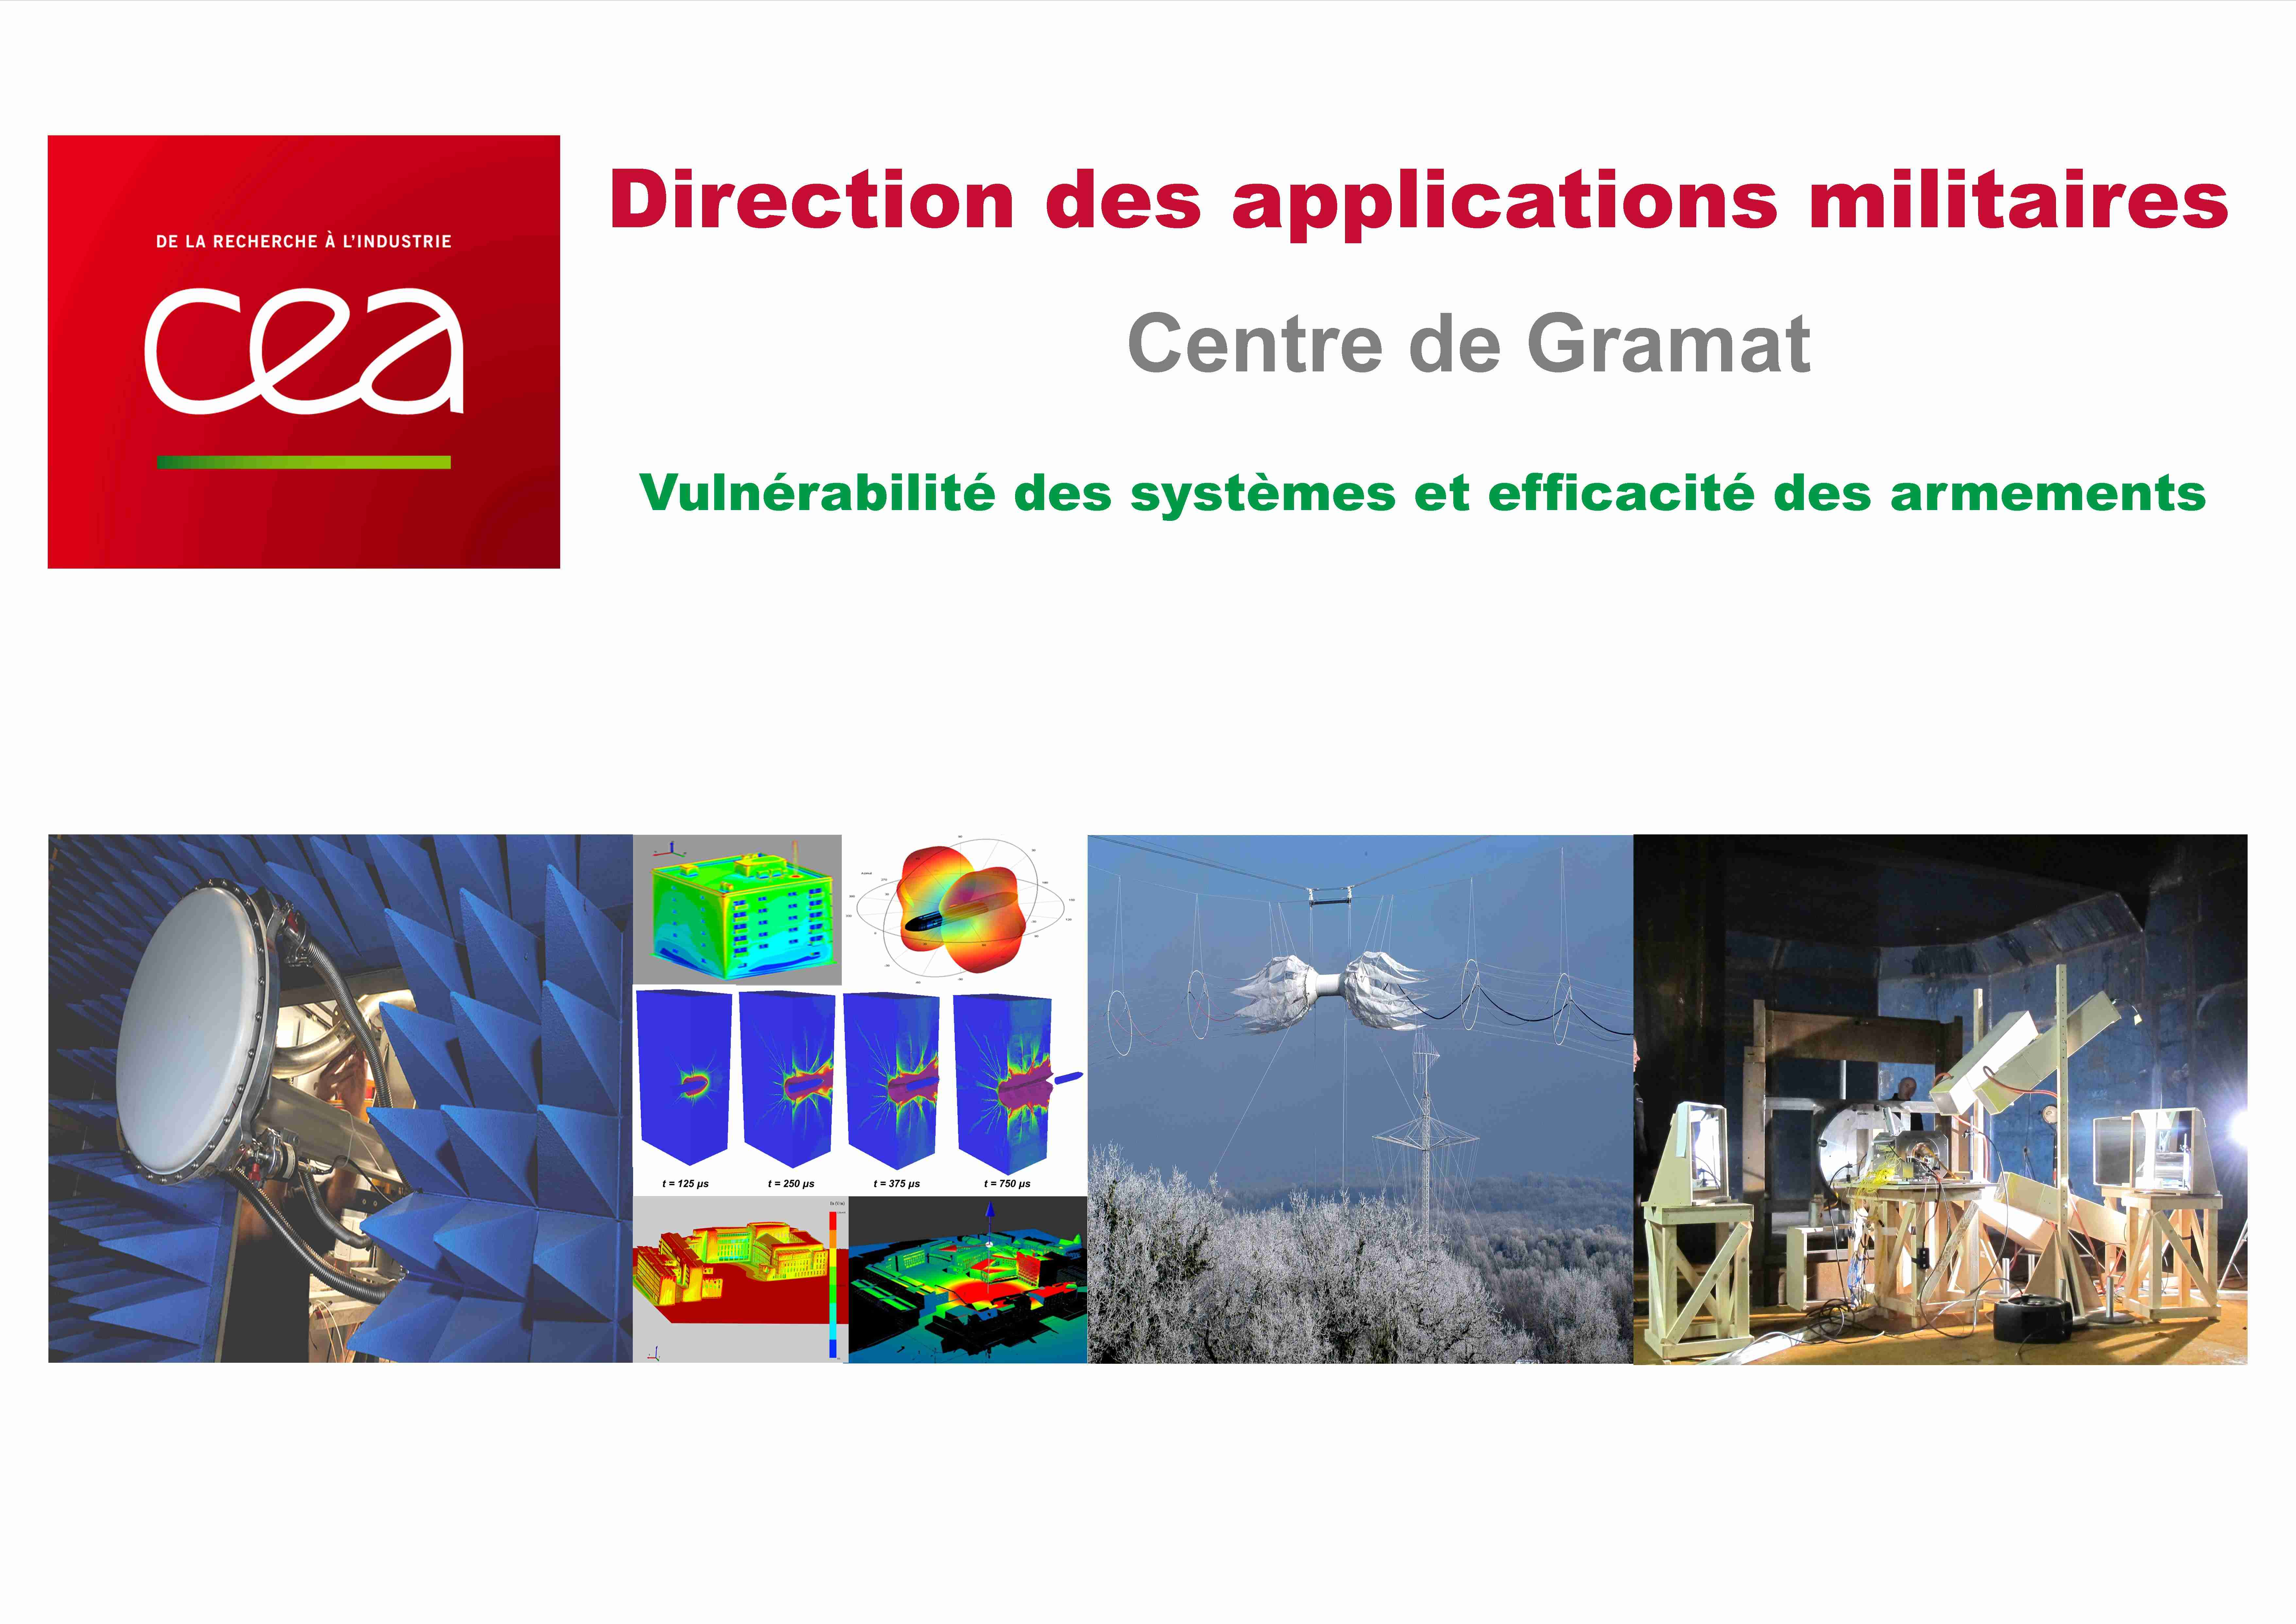
\includegraphics[width=11.5cm]{fichier_configuration/image_une_LQ}

\vspace{0.8cm}
\textcolor{darkgreen}{\large\textbf{ \@author{}}} \\

\vspace{1cm}

\color{darkgreen}

\begin{tabular}{llm{8cm}}

\textbf{Tuteur entreprise} &: & \textbf{\tuteurCEA} \\ 

\textbf{Tuteur enseignant}& : & \textbf{\tuteurecole}\\ 

& & \\ 

\textbf{Dates de mission} &: & \textbf{\datesstage} \\ 

\textbf{Formation suivie} &: & \textbf{\formation}\\ % type de master
\textbf{Etablissement} &:  & \textbf{\ecole} \\ % nom de l'ecole
\end{tabular} 

\vspace{1cm}

\textbf{Alternance effectuée au CEA/GRAMAT}


\end{center}
\end{titlepage}


\newpage
\pagestyle{empty}

\chapter*{}
\begin{center}
\textbf{Rapport de Mission}
\end{center}
\begin{center}
\begin{tabular}{|m{3.1cm}|m{4cm}|m{4cm}|}
\hline 
\rowcolor{darkred}
\multicolumn{3}{|c|}{\textbf{Visa de l'entreprise}} \\ 
\hline
\begin{center}
 \textbf{Entité}
 \end{center} & \begin{center}
 \textbf{Date}
 \end{center} & \begin{center}
 \textbf{Visa}
 \end{center} \\ 
\hline
\begin{center}
Tuteur entreprise : \tuteurCEA % tuteur CEA
\end{center}&  &  \\ 
\hline 
\begin{center}
 Chef de Laboratoire : \cheflabo
 \end{center} &  &  \\ 
%\hline 
%\begin{center}
% Responsable de l’unité de communication et affaires publiques (UCAP)  : PUECH Roland
% \end{center} &  &  \\ 
\hline 
\end{tabular} 
\end{center}


%\begin{center}
%\begin{tabular}{|m{4cm}|m{4cm}|}
%\hline 
%\rowcolor{darkred}
%\multicolumn{2}{|c|}{\textbf{Diffusion}} \\ 
%\hline
%\begin{center}
% \textbf{Entité}
% \end{center} & \begin{center}
% \textbf{Nombre d'exemplaires}
% \end{center} \\ 
%\hline
%\begin{center}
%Tuteur de Stage : \tuteurCEA % tuteur CEA
%\end{center}&  1  \\ 
%\hline 
%\begin{center}
%Tuteur enseignant : \tuteurecole %tuteur ecole
%\end{center}&  1  \\ 
%\hline
%\begin{center}
%Stagiaire : \auteurrapport % stagiaire 
%\end{center}&  1  \\ 
%\hline  
%\begin{center}
% Chef de Laboratoire : \cheflabo
% \end{center} &  1  \\ 
%\hline 
%\end{tabular} 
%\end{center}
\vspace{3cm}
\section*{Diffusion :}
\begin{itemize}
\item{\tuteurCEA : 1 ex.} 
\item{\tuteurecole : 1 ex.}
\item{\auteurrapport : 1 ex.}
\item{\cheflabo : 1 ex.}
%\item{UCAP : 1 ex.}
\end{itemize}

	% page de garde + verso blanc

		% Entête et pieds de page
	\pagestyle{fancy}% Indique que le style de la page sera justement fancy
	\renewcommand{\chaptermark}[1]{%
	\markboth{\MakeUppercase{\thechapter. #1}}{}}	
	\renewcommand{\footrulewidth}{0pt}	
	\renewcommand{\headrulewidth}{0.3pt}	
	\fancyfoot[L]{} %gauche du pied de page
	\fancyfoot[R]{} %m ilieu du pied de page
	\fancyfoot[C]{\thepage} %droite du pied de page
	\fancyhead[LO,RE]{
\includegraphics[scale=0.04]{fichier_configuration/logo-cea.png}}
	\fancyhead[RO,LE] {\leftmark}

\pagestyle{empty}

\chapter*{Remerciements}
%\addstarredchapter{Remerciements}

Je remercie tout d'abord Antoine Osmont pour m'avoir accueilli dans son excellent laboratoire. Merci aussi pour m'avoir expliqué différentes problématiques sur lesquelles j'ai travaillé avec toujours autant de clarté.

Je tenais ensuite à remercier Marc Genetier pour ses conseils et pour m'avoir aidé à résoudre les différents problèmes auxquels j'ai pu faire face. Merci aussi pour m'avoir aidé pour ce rapport, à la fois pour les différents informations sur Siame et pour les corrections et améliorations à y apporter. 

Je voulais aussi remercier Brigitte Martegoutte pour avoir pris le temps de m'expliquer comment se déroule les demandes d'achat au CEA. 

Je tiens enfin à remercier tous les membres du LDT pour leur excellent accueil et les discussions toujours aussi intéressantes. Merci donc à Sébastien, Laurent, Annise, Marie, Maryse, Nicolas, Noisette, Alexandre, Gérard, Emmanuel, Gregory, Guillaume, Valentin, Corentin, Jérémi, Antoine, Joanne et Azad.
	    % 




\tableofcontents	% table des matieres
\addstarredchapter{Sommaire}
\pagenumbering{arabic}

\chapter*{Introduction}

\addstarredchapter{Introduction}

Ce document a pour but de présenter la gestion d'un projet de sous-traitance de développement informatique au CEA. Nous traiterons plus spécifiquement de la façon dont la mise en place de l'architecture de Siame a été sous-traitée à Dev101. Les différentes phases du projet, les couts et les durées seront examinés. Nous suivrons le projet de la phase d'analyse à la rétrospective en passant par l'appel d'offre.

Une présentation plus complète de l'entreprise peut être trouvée dans mon premier rapport.

		% introduction

\pagestyle{fancy}

%\chapter{Présentation générale du CEA}
\pagenumbering{arabic}

\section{Le CEA}
\subsection{Généralités}
Le CEA (Commissariat à l’\' Energie Atomique et aux \' Energies Alternatives) est un établissement public industriel et commercial (EPIC) de droit privé. Ce statut lui permet d’avoir des activités avec différentes sociétés privées ou publiques tout en étant financé par l’état français. 
Le CEA a été créé en 1945 par l’ordonnance du général Charles De Gaulle. Il a pour but de réaliser les recherches sur le nucléaire et d'acquérir la maîtrise de l'atome. Il intervient ainsi dans quatre grands domaines de recherche : la défense, les énergies décarbonées, les technologies pour l’information et la santé, et la recherche fondamentale.
Il existe neuf centres de recherche CEA répartis sur le territoire français (Fig :\ref{centre_CEA}) (le centre Paris-Saclay comprend les sites de Saclay et de Fontenay aux Roses). Certains de ces centres sont liés aux applications militaires et sont contrôlés par la DAM (Direction des Applications Militaires) et d’autres sont liés aux applications civiles. Six PRTT (Plates-Formes Régionales de Transfert Technologique – (Hauts de France-Lille ; Grand Est-Metz ; Provence-Alpes-Côte d’Azur-Cadarache Gardane ; Occitanie-Pyrénées Méditerranée-Toulouse ; Nouvelle-Aquitaine-Bordeaux ; Pays de la Loire-Nates) appartenant au Pôle Recherche Technologique du CEA (CEA Tech) ont été créées en région, elles se rajoutent aux deux « bases arrières » historiques du CEA Tech de Saclay et de Grenoble. 




%\newpage
\subsection{Les directions opérationnelles du CEA}


Ces neuf centres se divisent au sein de quatre directions qui se partagent les grands domaines de compétence du CEA (\textit{cf}. Fig.~\ref{centre_CEA}):

\textbf{La DEN} : Direction de l’Energie Nucléaire qui opère sur les systèmes nucléaires du futur, l’optimisation du nucléaire industriel et sur le développement et l’exploitation d’outils expérimentaux et de simulation.

\textbf{La DRT }: Direction de la Recherche Technologique, qui se concentre sur les micro et nanotechnologies, les nouvelles technologies de l’énergie et les nanomatériaux ainsi que sur les systèmes numériques intelligents.

\textbf{La DRF }: Direction de la Recherche Fondamentale qui réalise la recherche des effets et applications du nucléaire au médical (radiothérapie, marquage biomoléculaire, etc.) et qui effectue la recherche traitant des sciences de la matière.

\textbf{La DAM} : Direction des Applications Militaires qui est le pôle Défense et Sécurité du CEA. La DAM travaille sur les armes nucléaires, la propulsion nucléaire, la sécurité et la non-prolifération ainsi que sur la défense conventionnelle.


\begin{figure}[h]
\centering
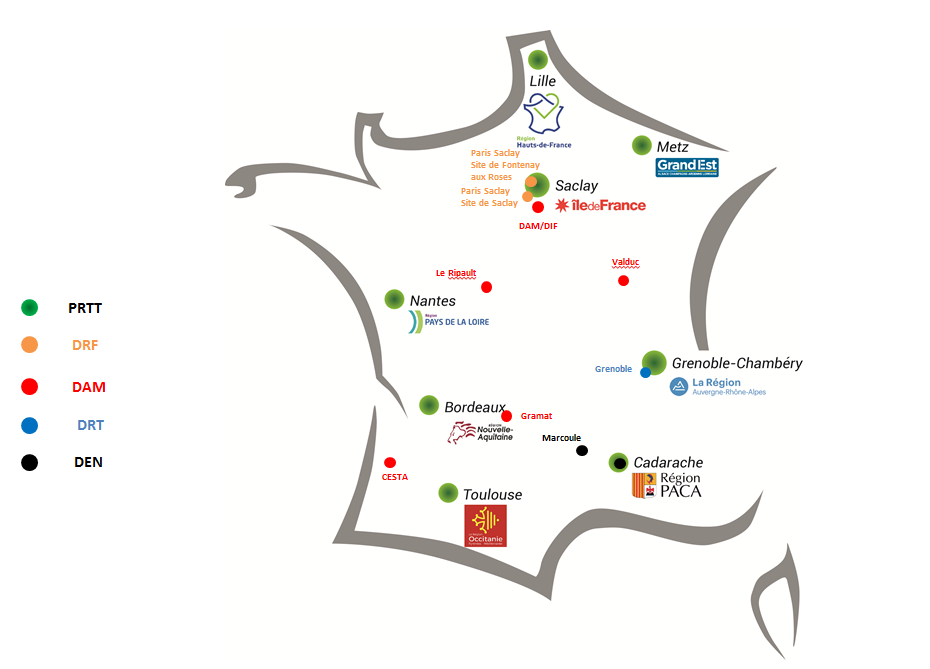
\includegraphics[scale=0.7]{fichier_configuration/carte_centres2018.png} 
\caption{Les centres CEA}
\label{centre_CEA}
\end{figure}
\FloatBarrier
\subsection{Le CEA en chiffres}

Le CEA était constitué, en 2017, de 33 laboratoires d'excellence, 27 équipes d’excellence et 3 initiatives d’excellence où travaillent 19 738 personnes (techniciens, ingénieurs, chercheurs et collaborateurs) soient 15 942 CDI, 1 183 doctorants, 160 post-doctorants, 554 alternants, 1 037 CDD et 862 autres salariées. Cela représente 5 milliards d’euros de budget (\SI{1.8}{\giga\euro} pour les activités défense, \SI{2.4}{\giga\euro} pour les activités civiles et \SI{0.8}{\giga\euro} pour les opérations assainissement et démantèlement), plus de 424 projets européens et 687 brevets en 2017 auprès de l’INPI (Institut National de la Propriété Industrielle) (4\textsuperscript{éme} place au niveau français derrière les industriels  Valéo, PSA et Safran et 1\textsuperscript{ère} place au niveau de organismes de recherche français).

\section{Le CEA/Gramat}

\subsection{Histoire du centre}

C’est en 1946 que le site de Gramat, situé au sein du parc naturel régional des causses du Quercy dans le Lot, est retenu pour implanter, dans le gouffre de Bèdes, des bancs d’essais de propulseurs de grande puissance (V2).

En 1956, le site devient le polygone d’expérimentations de la section atomique de la DEFA (Direction des Études et Fabrication d’Armement) et accueille les premiers essais liés au fonctionnement détonique des armes nucléaires.

En 1959, le site devient le CEG (Centre d’Etudes de Gramat), dépendant de la DGA (Délégation Générale pour l’Armement), puis, en 1965, les essais liés au fonctionnement détonique (non nucléaire) de l’arme nucléaire sont lancé. En 1965, des essais sur la dynamique des roches et les études de durcissement électromagnétique et mécanique sont mis en place.

C’est en janvier 2010 que le CEG de la DGA a rejoint le CEA. Il devient ainsi le dixième centre du CEA et le cinquième centre de la DAM.
Le site s’étend aujourd’hui sur 325 hectares et emploie 260 salariés ainsi que des stagiaires, apprentis et thésards. Il est le centre de référence pour l’étude de l’efficacité des armements et de la vulnérabilité des systèmes aux effets des armes conventionnelles et nucléaires.


\subsection{Domaine d'activité}

Les activités du CEA/Gramat se concentrent autour de trois domaines :
\begin{itemize}
\item{le nucléaire de défense (50~\%),}
\item{la défense conventionnelle (45~\%),}
\item{la sécurité globale (5~\%).}
\end{itemize}

Dans chacun de ces cas, le centre est spécialisé dans l’étude de la vulnérabilité des armes et systèmes de défense.

Le nucléaire de défense vise à étudier les effets du rayonnement, du souffle, du flash thermique et des ondes électromagnétiques générés par une arme.
Les recherches en défense conventionnelle permettent le développement des compétences en physique des explosifs, détonique, balistique terminale et en vulnérabilité des structures. La sécurité globale permet de mettre au profit de pouvoirs publics et de la sécurité des infrastructures, les compétences développées sur les deux points précédents. 

Enfin, la sécurité globale a pour objectif d’étudier la sécurité des infrastructures civiles ou militaires face aux actes malveillants, aux accidents ou aux catastrophes naturelles.

\subsection{Organisation de l'entreprise}

Le DEA (Département Effets des Armes) constitue l'organe principal de production technique du centre et est divisé en différents services, lesquels sont sous divisés en différents laboratoires (cf \textit{cf} Fig.~\ref{orga}). 

\begin{figure}[h]
\centering
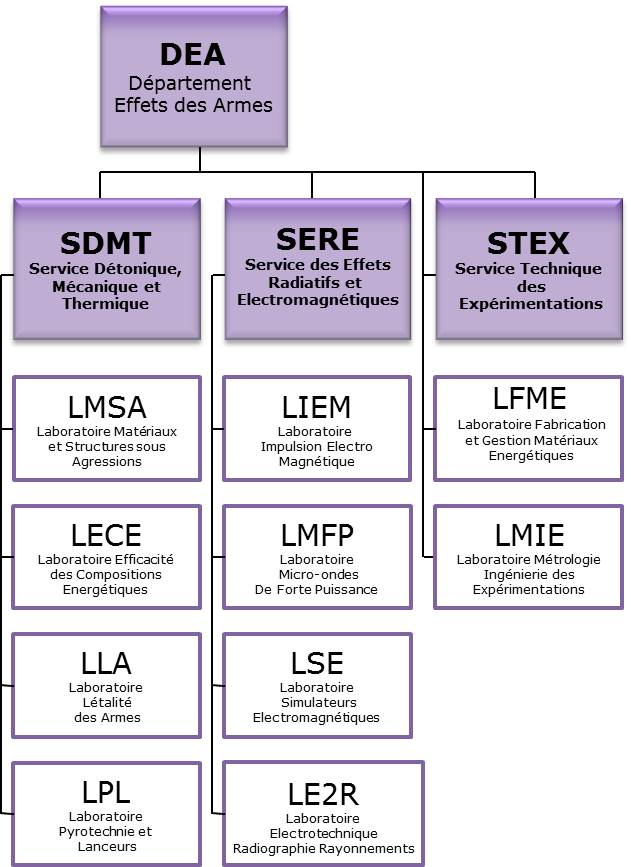
\includegraphics[scale=0.6]{fichier_configuration/organigramme.png} 
\caption{Organigramme du DEA du CEA/Gramat.}
\label{orga}
\end{figure}

\section{Positionnement dans l'entreprise}
\subsection{Besoins en logiciels du LECE}
Mon alternance se déroulera au Service Détonique, Mécanique et Thermique (SDMT) dans le Laboratoire  Efficacité des Compositions Énergétiques (LECE). Ce service travaille principalement sur l'effet des armes conventionnelles et les moyens de s'en protéger. Environ 70 personnes travaillent au SDMT, principalement des chercheurs et techniciens. La quinzaine de membres du LECE s'intéressent, eux, principalement à la modélisation et aux effets des explosifs. Dans le cadre de leur travaux, les chercheurs peuvent être amenés à développer des logiciels répondant à des besoins assez spécifiques.

C'est dans ce contexte que j'interviens au LECE. Plusieurs codes propres au laboratoire pourraient être améliorés. Les personnes travaillant sur ces codes sont principalement des ingénieurs chercheurs et n'ont pas forcément le temps et les compétences de s'occuper de la partie plus \og informatique \fg{} du logiciel.  

\subsection{Outils mis à disposition}
Pour des raisons de sécurité et de confidentialité, l'intégralité du matériel informatique mis à disposition est la propriété du CEA et il n'est pas possible d'utiliser du matériel personnel (PC, clef USB\dots{}). Il est aussi à noter que mon poste de travail est totalement déconnecté d'Internet. Il est donc très complexe d' installer des logiciels \og extérieurs \fg. Fort heureusement le centre fournit des services et logiciels suffisant pour que je puisse travailler dans de bonnes conditions : 
\begin{itemize}
\item un poste fixe sous Windows;
\item un accès à toutes les ressources du réseau interne (stockage distant, intranet, mail interne...);
\item le pack Office, TexMaker et d'autres outils \og bureautique \fg;
\item python 2.7 32~bits et Python 3.3 64~bits avec l'IDE Spyder;
\item des compilateurs C, C++ et Fortran 64~bits pour Windows et Linux;
\item un accès SSH à des machines Linux;
\item un serveur Git (GitLab) interne au CEA Gramat;
\item un serveur SQL (MySQL) lui aussi interne au CEA Gramat;
\item un accès à des postes reliés à internet pour rechercher des informations.
\end{itemize}
Les outils mis à ma disposition sont suffisants pour remplir ma première mission et sans doute les suivantes. 
 	

\chapter{Contexte et besoin}
\section{Mon rôle au CEA}
Le CEA (Commissariat à l’Énergie Atomique et aux Énergies Alternatives) est un établissement public industriel et commercial (EPIC) de droit privé. Ce statut lui permet d’avoir des activités avec différentes sociétés privées ou publiques tout en étant financé par l’état français. Le CEA a été créé en 1945 sous l’ordonnance du général Charles De Gaulle. Il a pour but de réaliser les recherches sur le nucléaire et d’acquérir la maîtrise de l’atome. Il intervient ainsi dans quatre grands domaines de recherche : la défense, les énergies décarbonées, les technologies pour l’information et la santé, et la recherche fondamentale. 

C’est en 1946 que le site de Gramat, situé au sein du parc naturel régional des causses du Quercy dans le Lot, est retenu pour implanter, dans le gouffre de Bèdes, des bancs d’essais de propulseurs de grande puissance (V2). En 1956, le site devient le polygone d’expérimentations de la section atomique de la DEFA (Direction des Études et Fabrication d’Armement) et accueille les premiers essais liés au fonctionnement détonique des armes nucléaires. En 1959, le site devient le CEG (Centre d’Etudes de Gramat), dépendant de la DGA (Délégation Générale pour l’Armement), puis, en 1965, les essais liés au fonctionnement détonique (non nucléaire) de l’arme nucléaire commencent. En 1965, des essais sur la dynamique des roches et les études de durcissement électromagnétique et mécanique sont mis en place. C’est en janvier 2010 que le CEG de la DGA a rejoint le CEA. Il devient ainsi le dixième centre du CEA et le cinquième centre de la DAM. Le site s’étend aujourd’hui sur 325 hectares et emploie 260 salariés ainsi que des stagiaires, apprentis et thésards. Il est le centre de référence pour l’étude de l’efficacité des armements et de la vulnérabilité des systèmes aux effets des armes conventionnelles et nucléaires. Il dispose de nombreux moyen expérimentaux comme le lanceur Ares présenté en figure \ref{ares}, qui permet de mesurer le comportement de matériaux soumis à des agressions physique extrêmes.

\begin{figure}[h]
\centering
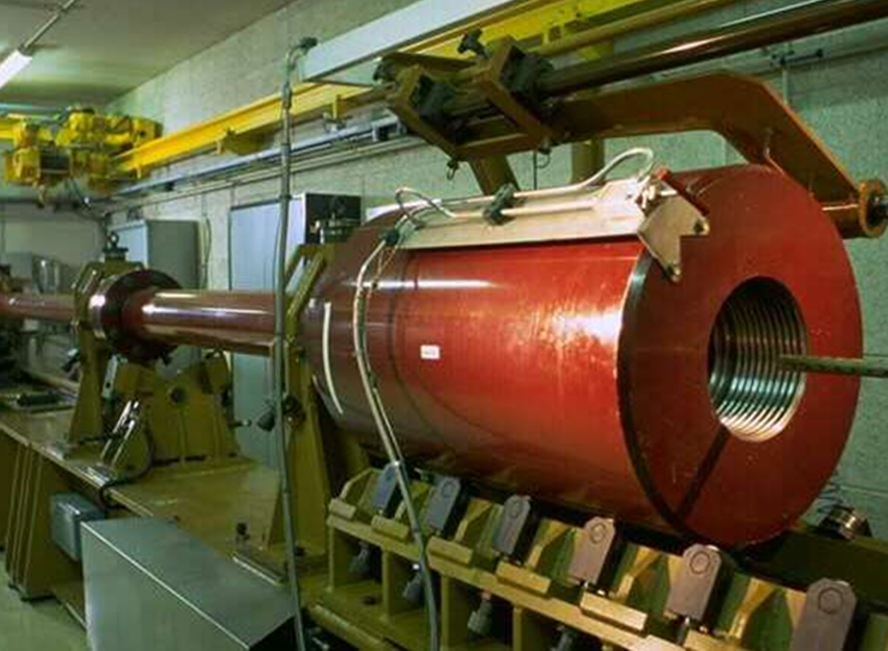
\includegraphics[scale=0.5]{ares.png}
\caption{Lanceur Arés} 
\label{ares}
\end{figure}

Dans le cadre de mon alternance, suis intégré dans le Service Détonique, Mécanique et Thermique (SDMT) au Laboratoire Détonique et Thermique (LDT).

La majorité des travaux du LDT portent sur la détonique. Il y a donc un fort besoin en applications spécifiques afin de répondre à des problématiques liées à la recherche. De nombreux logiciels sont développés en interne afin d'être au plus proche du besoin. Mon rôle est donc d'améliorer ces logiciels internes ou d'en développer des nouveaux. Je peux ainsi être amené à intervenir sur différentes étapes d'un projet, ou bien être responsable de l'intégralité d'un projet. 

\newpage

\section{Description de Siame}

Le centre d'étude dispose de nombreux codes de calcul et de simulation. Un de ces codes, Siame (SImulation Aérothermochimique de la Mécanique des Explosifs), a été principalement développé au laboratoire afin de répondre à des problématiques de défense. Il permet notamment d’obtenir des informations sur la composition et le comportement réactif d’un mélange de matériaux énergétiques dans un contexte thermodynamique. Ces informations peuvent par la suite être utilisées dans d’autre code de simulation pour décrire le comportement de différents matériaux. Siame est principalement utilisé par le CEA ainsi que par différents acteurs de la défense française. Une capture d’écran de l’IHM de Siame est présentée en figure \ref{screen}.

\begin{figure}[h]
\centering
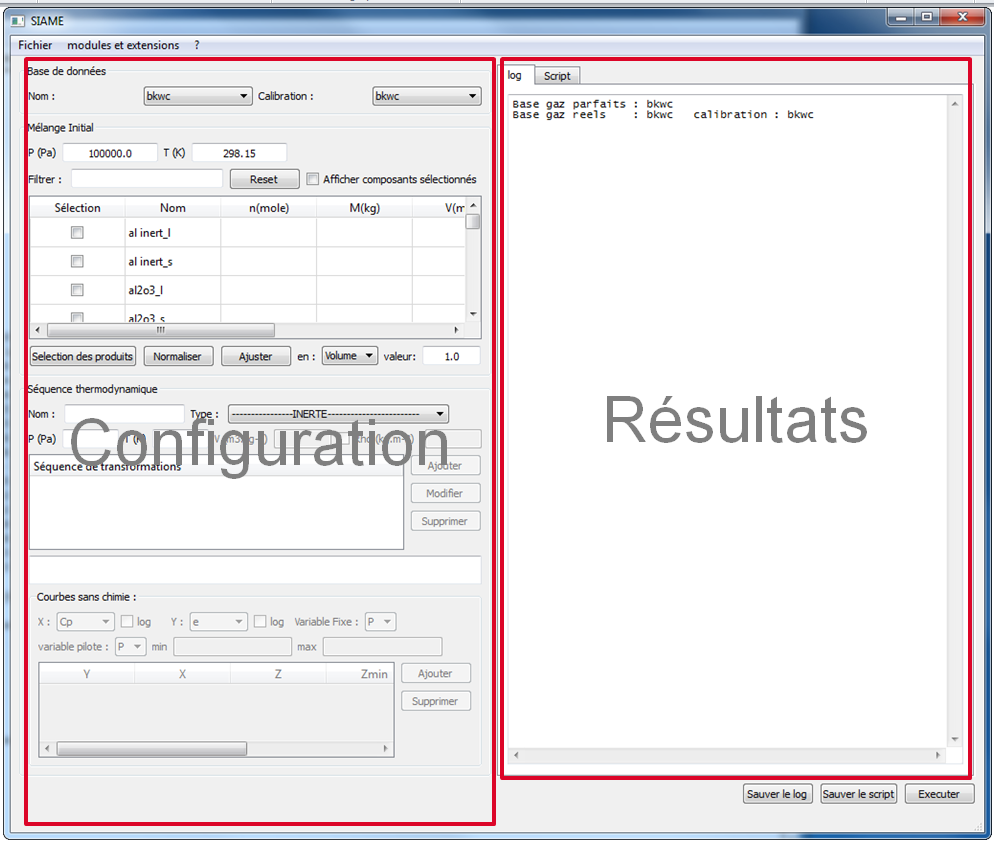
\includegraphics[scale=0.5]{Siame.png}
\caption{IHM de Siame} 
\label{screen}
\end{figure}

Siame est un programme écrit en plusieurs langages, principalement Python et Fortran. Ceci permet de combiner la flexibilité du Python avec la vitesse du Fortran. L'architecture très particulière de Siame sera détaillée ultérieurement. 

\begin{figure}[h]
\centering
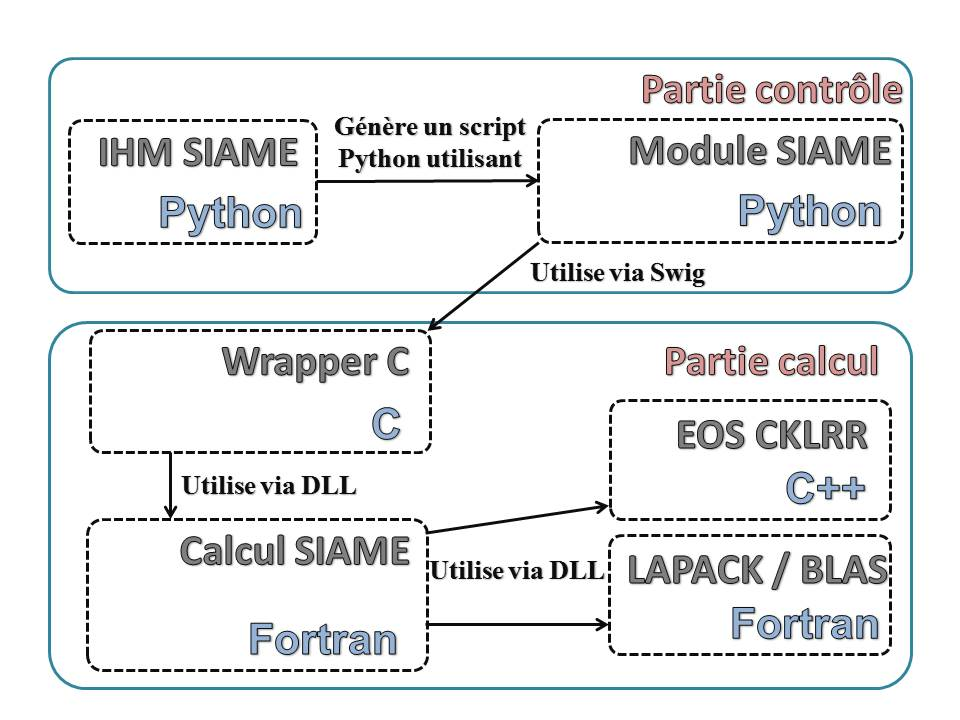
\includegraphics[scale=0.5]{SiameFonct.jpg}
\caption{Architecture de Siame} 
\label{archi}
\end{figure}

L'architecture si particulière est une des raisons principale pour lesquelles un sous-traitant est intervenu pour une partie du développement. Ce travail portera sur la façon dont a été gérée cette sous-traitance.

Les principales personnes qui ont été impliquées dans le projet sont Marc Genetier (Ingénieur Chercheur), Gérard Baudin (Ingénieur Chercheur) et Brigitte Martegoutte (Gestion des achats). Les dates, nom d'entreprises et montants ne sont donnés qu'à titre indicatif. 

\section{Besoin en sous-traitance}

Comme vu dans la partie précédente, l'architecture de Siame est particulière. Les domaines d'expertise du laboratoire étant en détonique, la mise en place de ce type d’architecture n’est pas dans les missions premières du LDT. Une maquette intégrant la partie thermochimique du code a été développé en interne, et il a été décidé de sous-traiter la mise en place de l'architecture présentée en figure \ref{archi}.

Ce choix est tout à fait justifiable puisque la mise en place d'une architecture complexe est un problème purement informatique. La partie la plus \og développement logiciel \fg{} a été sous traitée afin de permettre aux chercheurs de se concentrer sur la partie physique et scientifique du problème. 

La partie maquette / preuve de concept a été réalisée en amont par les chercheurs du LDT, expert du domaine. La partie industrialisation / mise en place de l’architecture est sous traitée afin de profiter des compétences d’entreprises spécialisées dans le développement d’applications scientifique. Une fois la version industrialisée opérationnelle, les chercheurs peuvent se servir de cette nouvelle version plus performante et y ajouter de nouvelles fonctionnalités. 

\chapter{Gestion du projet}

Le tableau \ref{chrono} présente une frise chronologique résumant les points clefs de la sous-traitance. 

\begin{table}[h]
\caption{Frise chronologique}
\label{chrono}
\centering
\begin{minipage}[t]{.7\linewidth}
\color{gray}
\rule{\linewidth}{1pt}
\ytl{01/13}{État des lieux codes de thermochimie}{teal}
\ytl{03/13}{Début du développement de la maquette}{teal}
\ytl{04/14}{Limites de la maquette atteinte}{teal}

\ytl{05/14}{Lancement d'appel à la concurrence}{cyan}
\ytl{06/14}{Début des négociations}{cyan}
\ytl{09/14}{Fin des négociations : Dev101 remporte le marché}{cyan}

\ytl{12/14}{1\textsuperscript{ére} livraison}{blue}
\ytl{05/15}{2\textsuperscript{éme} livraison}{blue}
\ytl{07/15}{3\textsuperscript{éme} livraison}{blue}
\ytl{08/15}{4\textsuperscript{éme} livraison}{blue}
\ytl{09/15}{5\textsuperscript{éme} livraison}{blue}
\ytl{10/15}{Fin du développement et début utilisation}{blue}

\ytl{10/16}{Fin garantie}{violet}

\rule{\linewidth}{1pt}%
\end{minipage}%
\end{table}


\section{Les débuts du projet}

Le projet Siame à commencer à voir le jour en début d'année 2013 avec un état des lieux des codes de thermochimie. Le principal programme répondant aux besoins du CEA est un code de thermochimie américain de nom de Cheetah. Ce programme présente cependant plusieurs défauts, notamment le fait qu'il soit impossible de le modifier ou de rédiger les simulations sous forme de script. Il n'a donc pas été jugé suffisant pour les besoins de la défense. La décision a alors été prise de développer un code de thermochimie français, du nom de Siame.

Siame a tout d'abord été écrit en Python comme une preuve de concept. Le développement de cette maquette s'est terminé début 2014 lorsque les temps de calculs sont devenus beaucoup trop longs. Le fait que la maquette montrerait ses limites et que le passage à un langage plus adapté serait nécessaire a toujours été prévu et il a été décidé de sous traiter ce changement. 

Le CEA est un pouvoir adjudicateur de la commande publique. Cela signifie qu'il est habilité à passer des marchés au nom de l'état. Les marchés entre 40 000 et 214 000€ sont donc publiés sur un site spécialisé accessible au grand public. Les principes qui régissent ces marchés sont le libre accès à la demande (offres en libre accès), la transparence (communiquer sur les raisons qui entrainent le rejet d'une offre) et l'égalité de traitement entre les concurrents (accès aux mêmes informations).


Un avis d’appel public à la concurrence a donc été publié en ligne. Ce document présente de manière succincte le besoin et spécifie principalement les modalités de candidature. On y apprend par exemple que le CEA accorde une grande importance à la capacité financière des entreprises partenaires. Des extraits de bilan des trois dernières années et le chiffre d’affaires sont demandés aux candidats et comptent pour une part importante de l’attribution de marché. 

Un cahier des charges de 18 pages est aussi publié afin de spécifier le besoin et clarifier le résultat attendu. On y trouve d’une part des informations sur le côté scientifique du projet comme le principe d’un code de thermochimie et des détails quant aux différents modèles à utiliser. On y retrouve aussi des points plus techniques comme les systèmes d’exploitation sous lesquelles la solution doit fonctionner ou des détails de l’IHM. Il présente pour finir des points de gestion de projets comme les exigences de garantie de la part du CEA, les modalités d’appréciation des livrables fourni par le sous-traitant ou encore les jalons clefs.


Le CEA exige que le projet soit facturé de manière forfaitaire et non pas au prorata du temps passé et qu'il soit composé d’une tranche ferme et de tranche optionnelle. La tranche ferme est composée d’une version fonctionnelle et assez complète des fonctionnalités de la maquette. Elle permet de faire toutes les simulations importantes et d’être interfacable avec d’autres applications. Un schéma décrivant les différentes fonctions de la tranche ferme est présenté en figure \ref{ferme}. La tranche optionnelle contient notamment des possibilités de simulations plus avancées et une IHM. 

\begin{figure}[h]
\centering
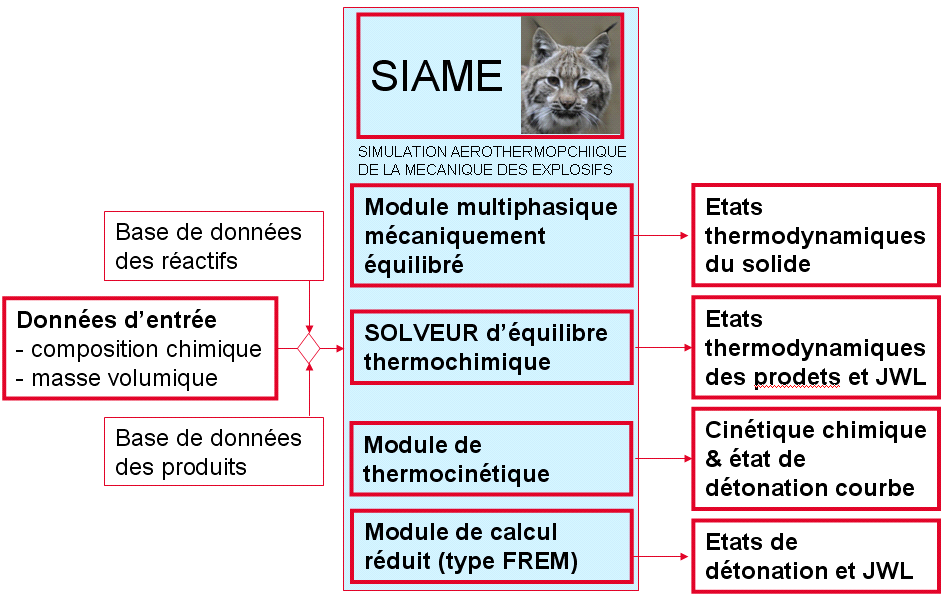
\includegraphics[scale=0.5]{siame_cahier_ext.png}
\caption{Description de la tranche ferme} 
\label{ferme}
\end{figure}

Le service des achats a publié la demande en mai 2014 et s'est occupé de la réception des candidatures.

\section{La gestion de la sous-traitance}
 
 Au total, 5 entreprises ont été intéressées par l'appel d'offre initial. Elles sont toutes des entreprises de taille considérable spécialisée dans le développement logiciel. Au final seul deux d'entre elles ont fait une offre, Dev202 et Dev101. Des réunions de négociation ont ensuite été réalisées afin de préciser le besoin et de discuter du prix. Le résultat de ces négociations peut être trouvé dans le tableau \ref{ref_prix} 
 
\begin{table}[h]
\caption{Récapitulatif des couts}
\label{ref_prix}
\begin{tabular}{l|lll|lll}
              &  \multicolumn{3}{c}{Dev101}       & \multicolumn{3}{c}{Dev202}               \\
             Tranche &  Ferme &  Optionnelle & Total &  Ferme & Optionnelle & Total \\
              \hline
Tarif initial (€) & 74358        & 42300             & 116658   &      83550         &      39094 & 122644 \\
Tarif négocié (€) &         59613     &        37737            &   97350    &      85627         &        37705            &      123332
\end{tabular}
\end{table}

L'entreprise Dev101 a remporté le marché car moins onéreuse pour une prestation similaire. Le cout total du projet est d’environ 100 000€ car la tranche fixe et la tranche optionelle ont été retenues.

Le CEA a accompagné Dev101 dans le développement de l’application. La mise à disposition de la preuve de concept leur a permis d’avoir une idée du résultat attendu et la preuve que ce résultat est atteignable. Beaucoup de documentation scientifique pertinente a été fourni afin que Dev101 puisse s’approprier la problématique. Des présentations ont été faites afin de spécifier dans les détails les méthodes de résolution appropriées. Une diapositive d’une des réunions de lancement est présentée figure \ref{reu_lancement}. On peut y voir le parallèle entre les différentes étapes de la simulation et le résultat attendu.

\begin{figure}[h]
\centering
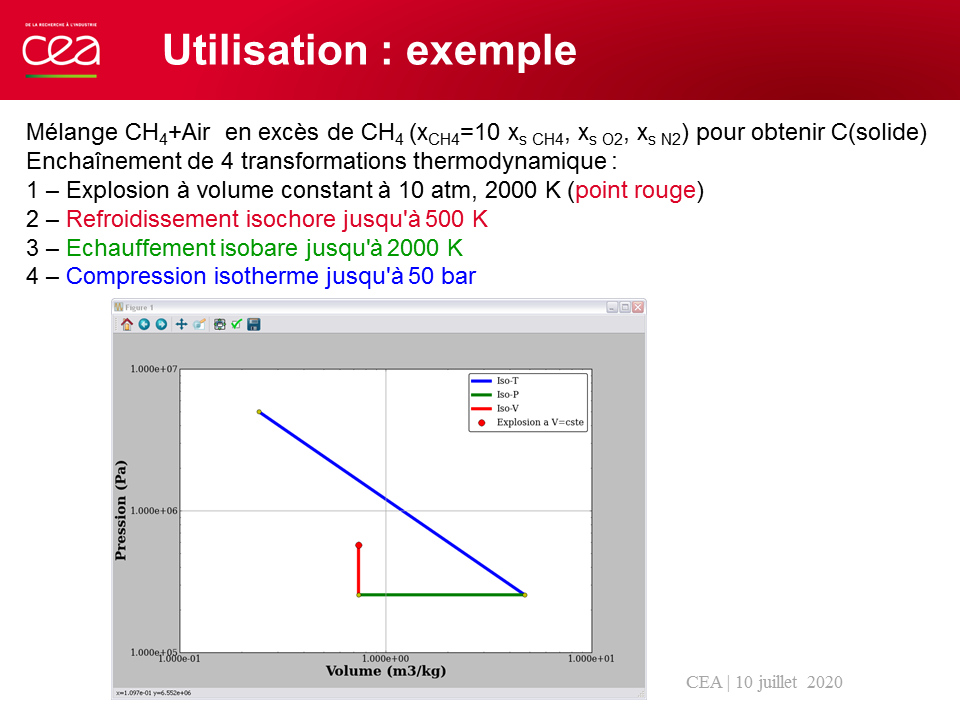
\includegraphics[scale=0.5]{demo_maquette.png}
\caption{Exemple résultat attendu} 
\label{reu_lancement}
\end{figure}

Dev101 à ensuite pu commencer à développer la solution et à la livrer. Au total 5 livraisons ont été effectuées sur un peu moins d’un an. Voici une description rapide de ce que contient chaque livraison : 
\begin{enumerate}
\item Implantation du noyau principal (19 656€) ;
\item implantation équation d’état (39 957€) ;
\item IHM (10 359€) ;
\item fonctionnalités supplémentaires (17 758€) ;
\item optimisation et portage (9 619€).
\end{enumerate}

Chaque livraison est suivie d’une courte phase de vérification. Durant cette phase, les membres du laboratoire peuvent tester le livrable, afin de vérifier qu’il est fonctionnel et correspond à la demande. Si ce n’est pas le cas, il est possible durant le mois suivant sa livraison, de signaler le problème à Dev101 afin que des corrections soient apportées.

Une fois la dernière livraison effectuée, une garantie d’un an commence. Cette garantie octroie un temps relativement long afin de détecter d’éventuels bugs et de les faire corriger. 5\%  du cout du projet est retenu jusqu'à la fin de cette garantie. Une fois la garantie expirée, le projet est considéré comme terminé et le solde de 5\% est payé au sous-traitant.

\section{Rétrospective}

Le projet s'est dans l'ensemble bien déroulé et toute les parties concernées sont satisfaites. Tous les livrables sont fonctionnels et ont été produit dans des temps raisonnables. Cette réussite est en partie le fruit de l'étroite collaboration entre le CEA et Dev101 au cours du projet.

Ce TR m’a permis de m’intéresser à la gestion d’un projet d’un point de vue assez différent de celui dont j'ai l'habitude. J’ai pu voir les différents acteurs ainsi que les procédures qui sont mise en place au CEA pour sous-traiter des développements. Ceci m'a permis de voir la démarche mise en œuvre pour lancer un appel d'offre, sélectionner le prestataire le plus adapté et encadrer le déroulement du projet.







\chapter*{Conclusion}
\addstarredchapter{Conclusion}

La sous-traitance de l'industrialisation de Siame a été une phase clef du développement. Les compétences du LDT en thermochimie ont pu être mises pleinement à profit par la réalisation d'un code performant. Le projet continu d'évoluer aujourd'hui et de nombreuses fonctionnalités ont été ajoutés.		% conclusion


\end{document}
